% ------------------------------------------------------------------------------
% Este fichero es parte de la plantilla LaTeX para la realización de Proyectos
% Final de Grado, protegido bajo los términos de la licencia GFDL.
% Para más información, la licencia completa viene incluida en el
% fichero fdl-1.3.tex

% Copyright (C) 2012 SPI-FM. Universidad de Cádiz
% ------------------------------------------------------------------------------

En este capítulo se recoge la arquitectura general del sistema de información,
el diseño de la interfaz de usuario, el diseño físico de datos, el diseño de
componentes software y la parametrización del software base.

\section{Diseño de la arquitectura}
En esta sección se define la arquitectura general del sistema de información,
especificando las distintas particiones físicas del mismo, la descomposición
lógica en subsistemas de diseño y la ubicación de cada subsistema en cada
partición, así como la especificación detallada de la infraestructura
tecnológica necesaria para dar soporte al sistema de información.

\subsection{Arquitectura física}

En este apartado, describimos los principales componentes hardware que forman la
arquitectura física de nuestro sistema, recogiendo por un lado los componentes
de servidor y los componentes de sistemas externos con los que colabora nuestro
sistema y por otro, los componentes hardware de cliente.

Este proyecto no precisa de una configuración física específica para su
funcionamiento, ya que se trata de un plugin para proyectos Django. Bastará
únicamente un servidor que cumpla con los requisitos mínimos necesarios para
alojar proyectos Django (para más información, se puede consultar la
documentación oficial en la web del proyecto Django \cite{djangobib}). Es más,
esta configuración dependerá en toda medida del proyecto Django donde se hará
uso de este plugin, ya que este será el que marque principalmente los requisitos
mínimos de los sistemas físicos, en función de su carga de trabajo,
disponibilidad, capacidad de respuesta u otros requisitos impuestos para dicho
software.

\subsection{Arquitectura lógica}
La arquitectura lógica del sistema está formada por los elementos software
(servicios, aplicaciones, librerías, frameworks, etc.) que componen el software
base, más el software desarrollado para cumplir los requisitos de la aplicación.
También, se recogen los componentes de sistemas externos con los que interactúa
nuestro sistema, así como los componentes software del lado cliente.

De esta forma, en este apartado de arquitectura lógica, vamos a describir todos
los elementos software que componen el software base de la aplicación, además
del propio software a desarrollar. De esta forma, podemos citar los siguientes
componentes software:
\begin{itemize}
    \item Primeramente, como acabamos de comentar, nos encontramos el elemento
        software que compone a nuestro proyecto, que no es más que un plugin
        para añadir a proyectos existentes, el cual permite al usuario la
        publicación de datos en internet siguiendo diferentes estándares
        conocidos.
    \item Este plugin está desarrollado, para un tipo de aplicaciones en
        concreto, aquellas que están desarrolladas haciendo uso del framework
        Django, por lo que el plugin está desarrollando de igual forma, haciendo
        uso de Django. Por lo que será necesario que la máquina posea una copia
        instalada de dicho framework.
    \item El framework Django, es un framework cuya finalidad es el desarrollo
        rápido de aplicaciones web, haciendo uso del patrón MVC. Este framework
        está desarrollado haciendo uso de la tecnología Python, por lo que es
        requisito indispensable que toda máquina en la que vaya a usarse dicho
        proyecto, tenga soporte para Python.
    \item A su vez, dicho proyecto estará alojado en algún servidor, ya sea
        Apache (nuestro caso, ) o cualquiera de los múltiples servidores
        disponibles a día de hoy. Un requisito de cualquiera de estos
        servidores, será el que tenga soporte para python (en el caso de Apache
        podemos usar mod\_python o wsgi).
    \item Por último, el sistema operativo donde se vaya a instalar todos los
        componentes anteriores, debe de tener soporte tanto para el servidor web
        donde vamos a incluir nuestro proyecto, como para la tecnología Python,
        ya que el resto de componentes comentados, funcionan sobre estas dos
        piezas. Por suerte, Python es un lenguaje de programación
        multiplataforma, el cual tiene soporte para los principales sistemas
        operativos existentes en la actualidad. Además, existen multitud de
        servidores web, como el comentado anteriormente (Apache), que poseen
        soporte también en los principales sistemas operativos existentes.
    \item En otro lugar, encontraremos aquellas tecnologías del lado del
        cliente, que también forma parte del proyecto o que intervienen en él.
        La tecnología que vamos a utilizar en el proyecto del lado del cliente
        es JavaScript. Se conoce por del lado del cliente, porque esto se
        ejecuta en la máquina del cliente, y no en el servidor. Además, también
        utilizaremos tecnologías como CSS para los estilos del proyecto.
\end{itemize}

A continuación, se muestra un gráfico (Figura \ref{fig:ArquitecturaLogica})
donde se puede apreciar mejor, las distintas capas que acabamos de describir
anteriormente, y cómo interactuarían estas entre ellas, desde el nivel más bajo
(el sistema operativo) hasta la capa capa más alta, compuesta por el proyecto
Django y el plugin que estamos desarrollando en este proyecto.

\begin{figure}[H]
    \begin{center}
        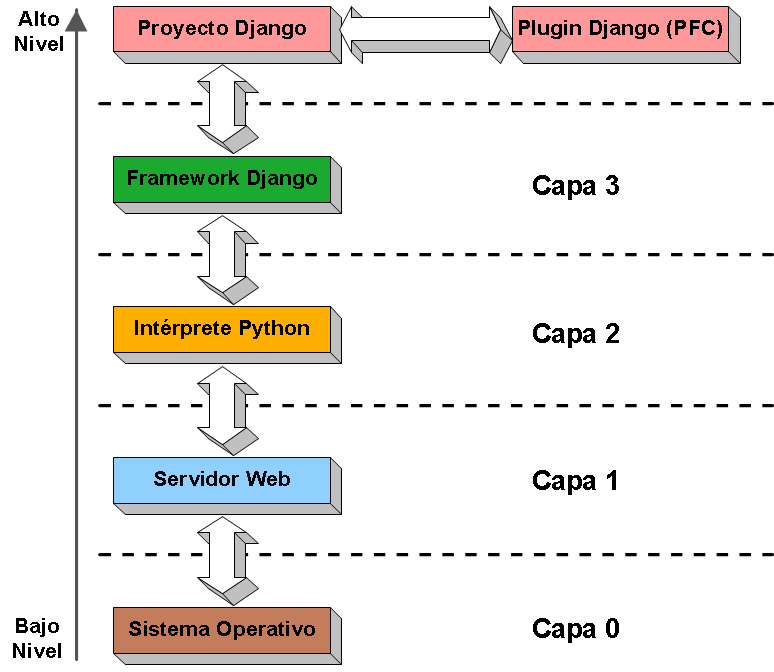
\includegraphics[width=1\textwidth]{disenio/arquitectura_logica.png}
    \end{center}
    \caption{Arquitectura lógica de cada uno de los elementos software}
    \label{fig:ArquitecturaLogica}
\end{figure}

\subsubsection{Estructura del proyecto}

Una vez que hemos visto como es la arquitectura lógica del proyecto, y en cada
una de las capas en las que podríamos definir el mismo, de forma que cada una de
estas interactúen únicamente con aquellas que están inmediatamente por encima o
por debajo de ella misma, toca describir en mayor profundidad la capa situada
más arriba de la jerarquía, la cual se corresponde a la aplicación que vamos a
desarrollar.

Toda aplicación contenida en un proyecto Django, posee una estructura común, de
forma que puedan identificarse cada uno de los elementos que componentes de
forma inmediata. Esta estructura se puede apreciar a modo orientativo, en la
Figura \ref{fig:ArquitecturaLogicaAplicacion}, donde se muestran cada uno de los
componentes principales de una aplicación. A continuación se describen la
finalidad de cada uno de estos apartados:
\begin{itemize}
    \item \textbf{Models:} se trata de un fichero llamado \textit{models.py} o
        un directorio llamado \textit{models}, el cual contendrá diferentes
        ficheros python, en donde se describirán cada uno de los modelos que
        componen a la aplicación Django.
    \item \textbf{Forms:} se trata de un fichero llamado \textit{forms.py} o un
        directorio llamado \textit{forms}, el cual contendrá diferentes ficheros
        python, en donde se describirán cada uno de los diferentes tipos de
        formularios Django.
    \item \textbf{Views:} se trata de un fichero llamado \textit{views.py} o un
        directorio llamado \textit{views}, el cual contendrá diferentes ficheros
        python, donde se describirán cada uno de los modelos que componen a la
        aplicación Django.
    \item \textbf{Templates:} se trata de un directorio común para todo el
        proyecto Django, en el cual se contendrán cada una de las plantillas las
        cuales se usarán por las vistas para mostrar la información en el
        formato especificado en la plantilla.
    \item \textbf{Static:} es un directorio donde se almacenan todos los
        elementos, tanto media, como estilos, javascript, etc\ldots que se
        usará en dicha aplicación.
    \item \textbf{Url's:} es un fichero llamado \textit{urls.py} o un directorio
        llamado \textit{urls}, que contendrá una serie de ficheros python, donde
        se definirán cada una de las URIs de las que dispondrá nuestro proyecto,
        y se asociarán con las vistas que se activará al llamar a dicha URI.
\end{itemize}

Estos componentes que hemos comentado son solo los principales, ya que además de
estos componentes, pueden existir muchos otros para otras finalidades.

\newpage

\begin{figure}[H]
    \begin{center}
        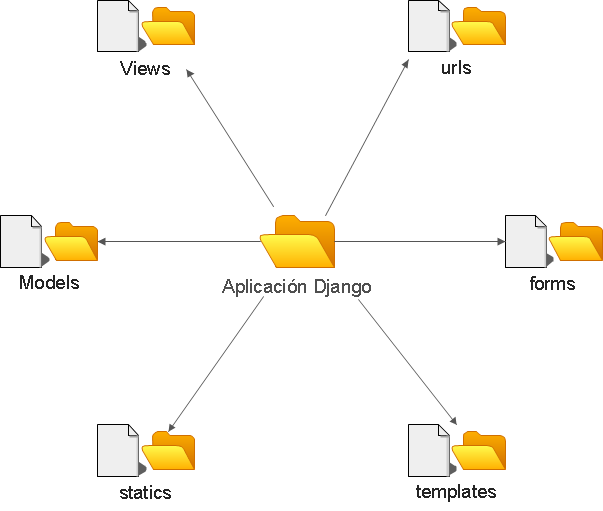
\includegraphics[width=0.95\textwidth]{disenio/arquitectura_logica_aplicacion.png}
    \end{center}
    \caption{Arquitectura lógica de una aplicación Django}
    \label{fig:ArquitecturaLogicaAplicacion}
\end{figure}


\subsection{Arquitectura de diseño}
La arquitectura de diseño especifica la forma en que los artefactos software de
más bajo nivel, interactúan entre sí para lograr el comportamiento deseado en el
sistema. Utilizaremos el patrón arquitectónico  Layers (Capas), con el cual
estructuramos el sistema en un número apropiado de capas, de forma que todos los
componentes de una misma capa trabajan en el mismo nivel de abstracción y los
servicios proporcionados por la capa superior utilizan internamente los
servicios proporcionados por la capa inmediatamente inferior.

Es este caso, para la realización del proyecto, estamos utilizando Django, que
se trata de un framework que aunque no lo sigue fielmente, está basado en el
patrón de diseño MVC (Modelo-Vista-Controlador), de tal forma que en toda
aplicación Django se hace una separación entre los distintos artefactos software,
los cuales interactuando entre sí, conforman el comportamiento esperado del
software. Por consiguiente, tal y como se aprecia en la figura de más abajo
(Figura \ref{fig:DjangoPattern}) podemos decir que toda la lógica de una
aplicación Django se encuentra dividida en los siguientes artefactos:
\begin{itemize}
    \item Los modelos.
    \item Las URL's.
    \item Las views (o vistas).
    \item Los templates (o plantillas).
\end{itemize}

\begin{figure}[H]
    \begin{center}
        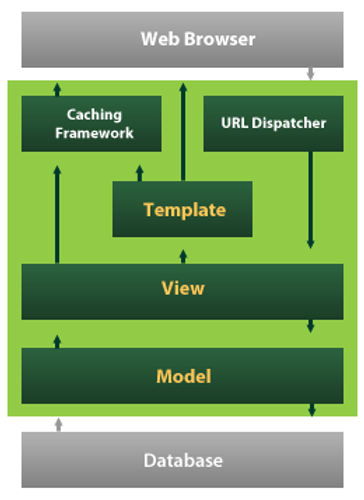
\includegraphics[width=0.6\textwidth]{disenio/esquema_django.png}
    \end{center}
    \caption{Patrón de diseño usado en el framework Django (fuente:
              \href{http://cambioderuta.wordpress.com/2010/01/11/\%C2\%BFque-es-django/}{Cambioderuta})}
    \label{fig:DjangoPattern}
\end{figure}

A continuación, vamos a relacionar cada uno de estos artefactos con la capa con
la que se corresponderían cada uno: presentación, negocio o integración.

\subsubsection{Capa de presentación}
Este grupo de artefactos software conforman la capa de presentación del sistema,
incluyendo tanto los componentes de la vista como los elementos de control de la
misma.

En el framework Django, esta capa se correspondería con los conocidos como
\textit{templates}. Mediante el uso de plantillas en Django, se consigue
separar la presentación de un documento, de la obtención y tratamiento de los
datos. En las plantillas se definen los rellenos y alguna lógica de control
básica para determinar como mostrar los datos. Mediante las plantillas de Django,
aunque el resultado más común pueda ser HTML, se puede generar cualquier tipo de
documento basado en texto, donde presentar los datos.
\subsubsection{Capa de negocio}
Este grupo de artefactos software conforman la capa de negocio del sistema,
incluyendo los elementos del modelo de dominio y los servicios (operaciones del
sistema).

En el caso del framework Django, la capa de negocio estaría fuertemente ligada
con los views (o las vistas, que se corresponden con los controladores en el
patrón MVC). En las vistas de Django, se lleva a cabo el tratamiento de los
datos, se consultan y se realizan operaciones de los mismos, y opcionalmente
estos se envían a la capa de presentación (los templates de Django) donde se
muestran al usuario. Si nos fijamos en la figura \ref{fig:DjangoPattern},
podemos ver, que los controladores hacen un poco como nexo de unión entre los
templates y los modelos (entre la capa de presentación y de integración).
\subsubsection{Capa de integración}
Este grupo de artefactos software conforman la capa de integración del sistema,
incluyendo las clases de abstracción para el acceso a datos (BD o sistema de
ficheros) o a sistemas heredados.

En esta capa, entran en juego diferentes elementos del framework Django.
Primeramente podríamos nombrar a los modelos, estos no son otra cosa, sino
clases Python, las cuales son una representación de las tablas que hay
almacenadas en la base de datos, junto con sus características (restricciones,
valores iniciales, etc), mediante esto se simplifica mucho la representación de
los datos para el usuario, ya que los tratará como objetos de una clase.

Por otro lado, aparecen los managers, estos elementos son una interfaz la cual
poseen todos los modelos de un proyecto Django (son configurables, ya que se
pueden crear interfaces que muestren solo ciertos datos), a través de la cual,
permite al usuario realizar consultas (desde sencillas hasta complejas), usando
un lenguaje propio de consulta del framework (evitamos tener que hacer uso de
SQL, aunque también puede utilizarse este). Con esto, llegamos a la tercera
característica, ya que al hacer uso de un lenguaje propio de consultas en Django,
estas son válidas para cualquier sistema de bases de datos soportado por Django
(este posee distintos backends para distintos motores de bases de datos), de
forma que una misma aplicación funcione con bases de datos PostgreSQL, Oracle,
etc \ldots sin necesidad de realizar cambios en las consultas.
\subsubsection{Servicios transversales}
Este grupo de artefactos software pueden ser usados por elementos de cualquiera
de las capas del sistema y fundamentalmente proporcionan servicios relacionados
con requisitos no funcionales (calidad).

Para nuestro caso, el framework Django posee determinadas características, las
cuales ayudan al cumplimiento de determinados requisitos no funcionales de los
que comentamos anteriormente (Sección \ref{sec:RQNF}), como son los siguientes:
\begin{itemize}
    \item \textbf{Seguridad:} Django incorpora la gestión automática de
        sesiones, o la generación automática de formularios basados el modelos o
        definidos por el programador, incorporando a su vez medidas de seguridad
        (como por ejemplo contra ataques csrf).
    \item \textbf{Mantenibilidad:} la herramienta promueve a la escritura de
        un código fácil de mantener, a parte de estructurar las aplicaciones en
        partes bien diferenciables, de forma que se puedan localizar los
        distintos elementos fácilmente por cualquier desarrollador con algo de
        experiencia en Django, promueve además el uso de patrones de diseño
        (como puede ser el patrón DRY, Facade, etc).
        
        Además, por otro lado, el desarrollo del proyecto, promueve un
        compromiso de seguir unos códigos de buenas maneras definidos en
        \cite{pep8}.
    \item \textbf{Portabilidad:} el framework está desarrollado en Python, el
        cual se trata de un lenguaje multiplataforma, de tal manera que la
        aplicación será válida en cualquier sistema que soporte Python.
\end{itemize}


\section{Diseño de la interfaz de usuario}

En esta sección vamos a proceder a detallar las interfaces que existirán entre
el sistema y el usuario de la aplicación, de forma que se pueda apreciar el
aspecto de estas y el comportamiento que mostrarán las mismas. De forma que sea
más fácil de apreciar para el lector, se van a realizar una serie de bocetos de
cada una de las interfaces, y sobre estos bocetos, se definirá el comportamiento
que tendrán.

Además, a continuación en la figura \ref{fig:mapa_web} se muestra el mapa de
navegabilidad de la aplicación, del cual se realizarán bocetos de las siguientes
interfaces:
\begin{itemize}
    \item Listado de namespaces.
    \item Visibilidad de modelos y atributos.
    \item Visualización de los modelos.
    \item Mapeo de modelos.
    \item Mapeo de los atributos. 
\end{itemize}

\begin{figure}[H]
    \begin{center}
        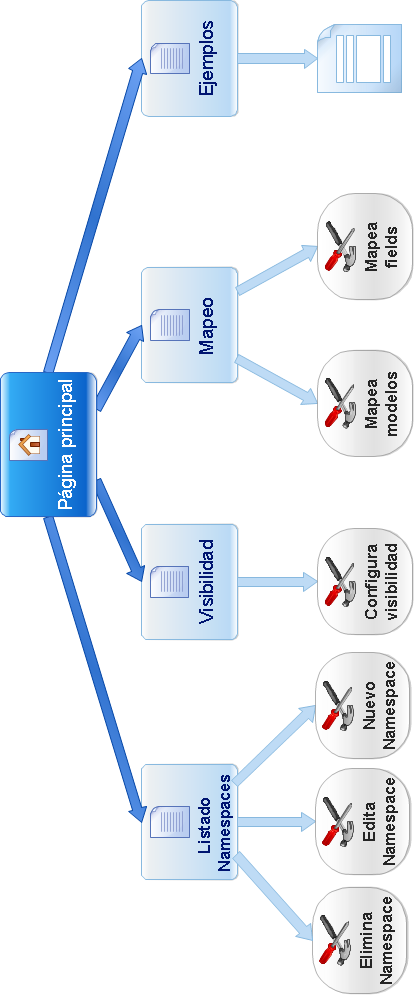
\includegraphics[width=0.45\textwidth]{disenio/mapa_web.png}
    \end{center}
    \caption{Mapa web de la aplicación}
    \label{fig:mapa_web}
\end{figure}

\subsection{Listado de namespaces}

A continuación en la figura \ref{fig:lista_namespaces} se muestra un boceto de
la interfaz para el listado de namespaces de la aplicación.

\begin{figure}[H]
    \begin{center}
        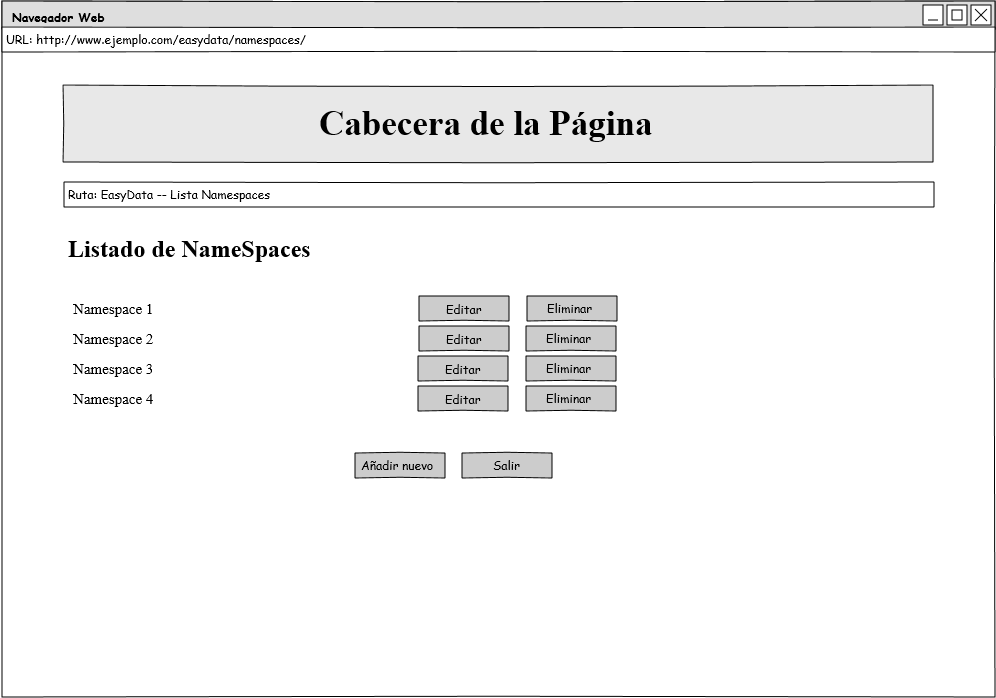
\includegraphics[width=1\textwidth]{mockups/lista_namespaces.png}
    \end{center}
    \caption{Boceto del listado de namespaces}
    \label{fig:lista_namespaces}
\end{figure}

Si observamos el boceto, podemos apreciar que se muestra un listado con cada uno
de los namespaces existentes en la aplicación, los cuales pueden utilizarse para
realizar la exportación de datos. Junto a cada uno de los nampesaces, aparecen
dos botones, los cuales permiten editar las propiedades o actualizar la
especificación de dicho namespace, o eliminar el mismo junto con todas sus
entidades y propiedades.

\subsection{Visibilidad de modelos y atributos}

A continuación en la figura \ref{fig:visibilidad} se muestra un boceto de
la interfaz para la configuración de la visibilidad de los modelos y los
atributos.

\begin{figure}[H]
    \begin{center}
        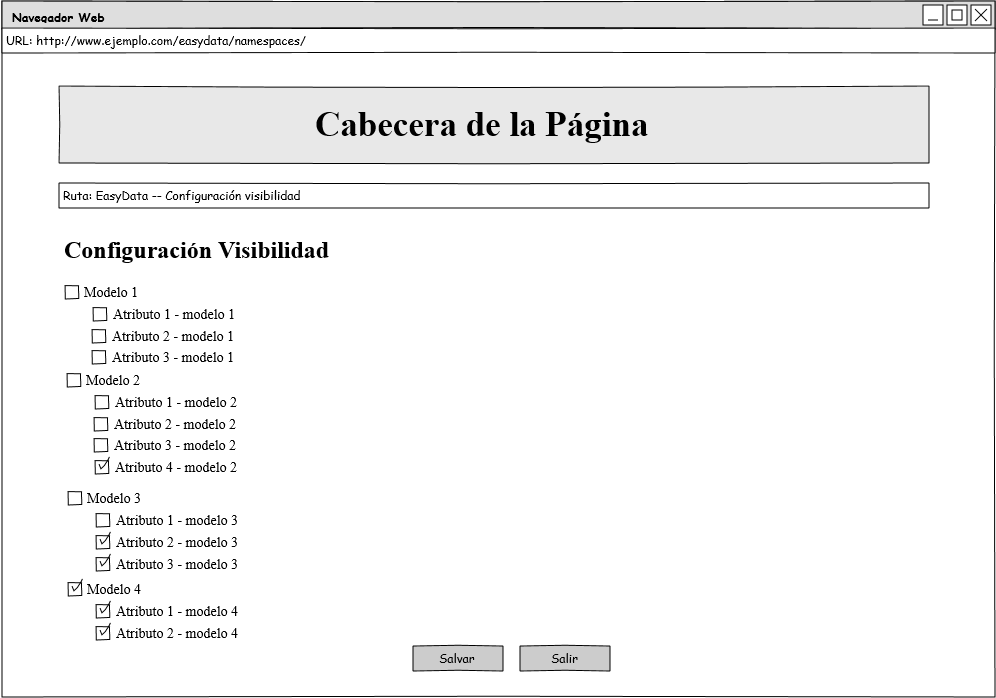
\includegraphics[width=1\textwidth]{mockups/visibilidad.png}
    \end{center}
    \caption{Boceto de la interfaz para la modificación de la visibilidad}
    \label{fig:visibilidad}
\end{figure}

Si observamos el boceto, la configuración de la visibilidad de los modelos y
atributos del proyecto es bastante sencilla. Se muestra al usuario por pantalla
un listado de todos los modelos y atributos que componen a cada uno de estos en
forma de árbol. El usuario marcará aquellos modelos o atributos de estos que
desee que sean visibles. De esta forma, si el usuario quiere que un modelo sea
completamente visible, marcará la casilla del modelo, y además marcará todos los
atributos del mismo. Por otro lado, si un usuario no desea que un determinado
atributo de un determinado modelo no sea visible, únicamente deberá dejar la
casilla correspondiente a dicho modelo sin marcar. Finalmente, si el usuario
desea que un modelo no sea visible, bastará con marcar la casilla
correspondiente al modelo, independientemente de los atributos del mismo que
estén o no marcados.

\subsection{Visualización Modelos}

A continuación en la figura \ref{fig:visualiza_modelos} se muestra un boceto de
la interfaz donde se podrá visualizar la configuración realizada del mapeo de
los diferentes modelos y atributos con los diferentes namespaces cargados en la
aplicación.

\begin{figure}[H]
    \begin{center}
        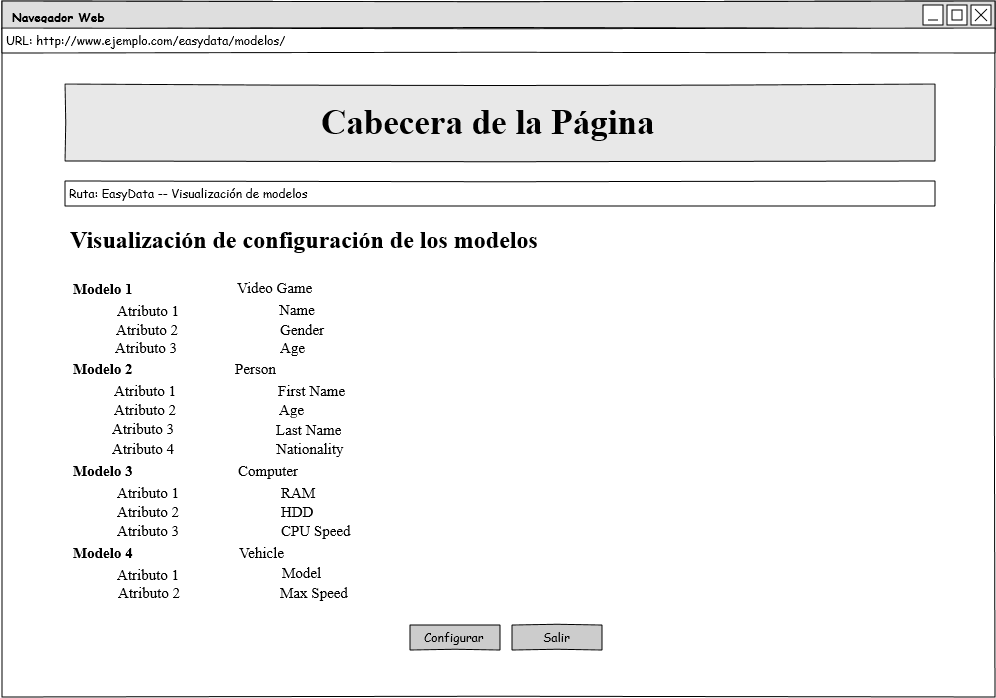
\includegraphics[width=1\textwidth]{mockups/visualiza_modelos.png}
    \end{center}
    \caption{Boceto de la interfaz para visualización del mapeo de los modelos}
    \label{fig:visualiza_modelos}
\end{figure}

Esta pantalla es plenamente informativa, dando al usuario una idea de la
configuración que existe actualmente del mapeo entre los modelos que componen su
proyecto y las entidades de los namespaces. Posteriormente, podrá modificarse la
configuración existente, pulsando sobre el botón \textit{Configurar}.

\subsection{Mapeo de los modelos}

En la figura \ref{fig:mapeo_modelos} de abajo, se muestra un boceto de la
interfaz para la configuración del mapeo de los modelos del proyecto, con las
entidades de los diferentes namespaces que queramos hacer que se corresponda.

\newpage

\begin{figure}[H]
    \begin{center}
        \includegraphics[width=1\textwidth]{mockups/mapeo_modelos.png}
    \end{center}
    \caption{Boceto de la interfaz para el mapeo de los modelos}
    \label{fig:mapeo_modelos}
\end{figure}

El usuario, cuando se encuentre en la pantalla del visualización de la
configuración del mapeo de los modelos, tal y como se indica en el punto
anterior, podrá acceder a configurar dicho mapeo, mostrándole la pantalla
que se puede apreciar, donde para cada uno de los modelos que posee el proyecto
donde se encuentra esta aplicación, mostrará las distintas entidades disponibles
para cada uno de los namespaces. Tras hacer la correspondencia, que el usuario
crea conveniente, solo tendrá que pulsar sobre el botón de salvar, para almacenar
los cambios realizados.

\subsection{Mapeo de los atributos}

En la figura \ref{fig:mapeo_atributos} que se muestra a continuación, podemos
apreciar un boceto de la interfaz que se usará en la aplicación para hacer
corresponder, cada uno de los atributos de los modelos de nuestra aplicación,
con cada posible propiedad de la entidad con la que se ha relacionado el modelo
al que pertenece el atributo, o con cualquiera de las propiedades de los
namespaces cargados.

\begin{figure}[H]
    \begin{center}
        \includegraphics[width=1\textwidth]{mockups/mapeo_atributos.png}
    \end{center}
    \caption{Boceto de la interfaz para el mapeo de los atributos}
    \label{fig:mapeo_atributos}
\end{figure}

Si nos fijamos bien, aparece una entrada por cada uno de los atributos de los
que dispone el modelo, y al lado de cada uno de estos, dos desplegables con cada
uno de los diferentes namespaces y cada una de las posibles propiedades con las
que podremos hacer corresponder al atributo. Una vez se haya realizado toda la
correspondencia, solo habrá que almacenar los cambios realizados pulsando sobre
el botón de salvar.


\section{Diseño de datos}
En esta sección definimos los datos que utilizará la aplicación, y como se
estructuran los mismos dentro de la base de datos. Para plasmar la estructura de
los datos en la base de datos, en la figura \ref{fig:modelo_conceptual} se
muestra el diagrama de datos, donde podemos apreciar cada una de las tablas y
columnas de las mismas existentes en la base de datos, así como las funciones
que implementan cada una de ellas.

\newpage

\begin{figure}[H]
    \begin{center}
        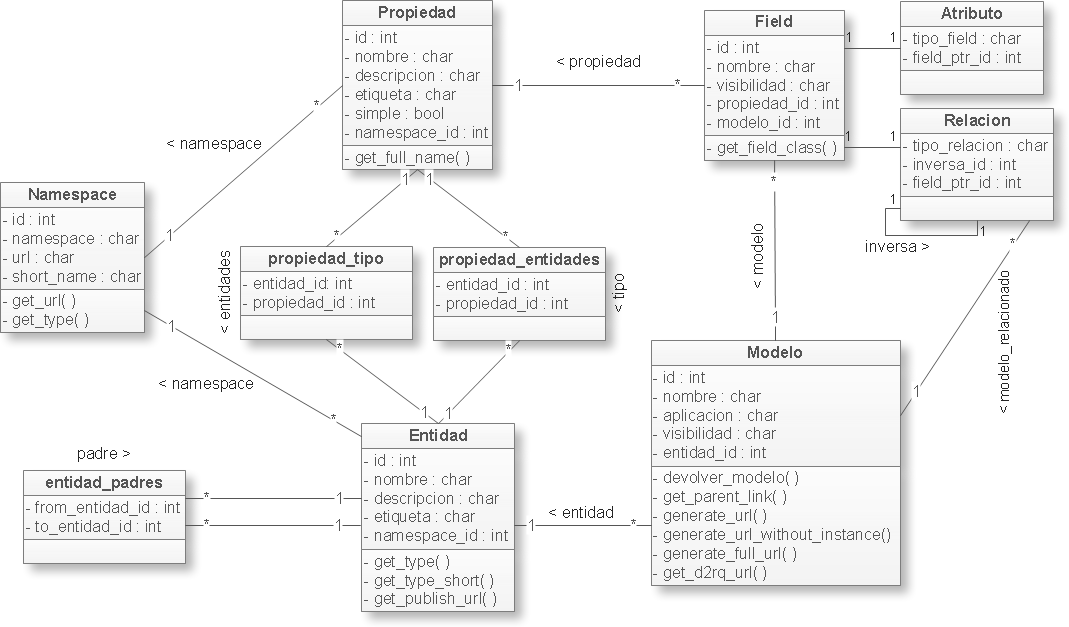
\includegraphics[width=1.0\textwidth]{disenio/modelo_conceptual.png}
    \end{center}
    \caption{Diseño de los datos}
    \label{fig:modelo_conceptual}
\end{figure}

A continuación se detallan cada una de las tablas que aparecen en el diagrama de
diseño de los datos:
\begin{itemize}
    \item \textbf{Namespace:} Esta tabla representa a un determinado namespace,
        almacenando el nombre del mismo y la url donde se encuentra el schema
        que describe cada una de sus entidades y propiedades.
    \item \textbf{Entidad:} Es una determinada entidad de un namespace.
        Almacena el nombre del mismo, y la etiqueta y descripción asociadas en
        el caso de que la posean. Está relacionada con cada una de las
        propiedades que lo componen, con el namespace al que pertenece y con los
        modelos con los que lo haga corresponder el usuario.
    \item \textbf{Propiedad:} Representa a una determinada propiedad de una
        entidad (no tiene que estar relacionado con una entidad forzosamente),
        almacenando el nombre y el tipo de la misma, así como una etiqueta y
        descripción que pueda tener asociados, al igual que en el caso de las
        entidades. Además, estará relacionada con la entidad y el namespace a la
        que pertenece y con los fields con los que lo haya hecho corresponder el
        usuario.
    \item \textbf{Modelo:} Es la representación de cada uno de los modelos de
        los que está compuesto el proyecto Django. Almacena el nombre del mismo,
        la aplicación del proyecto a la que pertenece y la visibilidad que
        tendrá el mismo respecto al exterior. Posee relaciones con la entidad
        con la que se haga corresponder y con los fields de los que está
        compuesto.
    \item \textbf{Field:} Esta tabla a su vez, representa a cada uno de los
        fields del proyecto, que componen a los modelos descritos anteriormente.
        Están compuestos por el nombre de estos y la visibilidad que tendrán
        respecto al exterior. Posee relaciones tanto con el modelo al que
        pertenecen, como con las propiedades con las que se haya hecho
        corresponder. Además, existen dos tablas más, llamadas Atributo y
        Relacion, con una relación OneToOne con la tabla Field (es la forma de
        expresar la herencia en Django), de tal forma que se indica si dicho
        field del modelo es un atributo o una relación.
    \item Las tablas entidad\_padres, propiedad\_entidades y propiedad\_tipo son
        tablas auxiliares que se utilizan para implementar las relaciones
        Muchos-A-Muchos en la base de datos, y los datos que contienen
        únicamente son los punteros (id) a los elementos que relaciona.
\end{itemize}

\section{Diseño de componentes}

En esta sección se definen los componentes software necesarios para la
implementación del sistema. Este sistema se implementa como una única aplicación
Django, pero se puede descomponer en subsistemas en función de las diferentes
funcionalidades que ofrece y de cómo se encontrará estructurado. Al estar
haciendo uso para la realización del proyecto de un framework basado en el
patrón MVC, vamos a diferenciar dentro del mismo, distintos módulos o
componentes, como son los modelos, los controladores y las vistas (conocidos por
modelos, vistas y plantillas respectivamente en Django). En la siguiente figura
(\ref{fig:componentes}) se puede ver un diagrama que refleja perfectamente la
estructura de los componentes que deberá de tener la aplicación.

\newpage

\begin{figure}[H]
    \begin{center}
        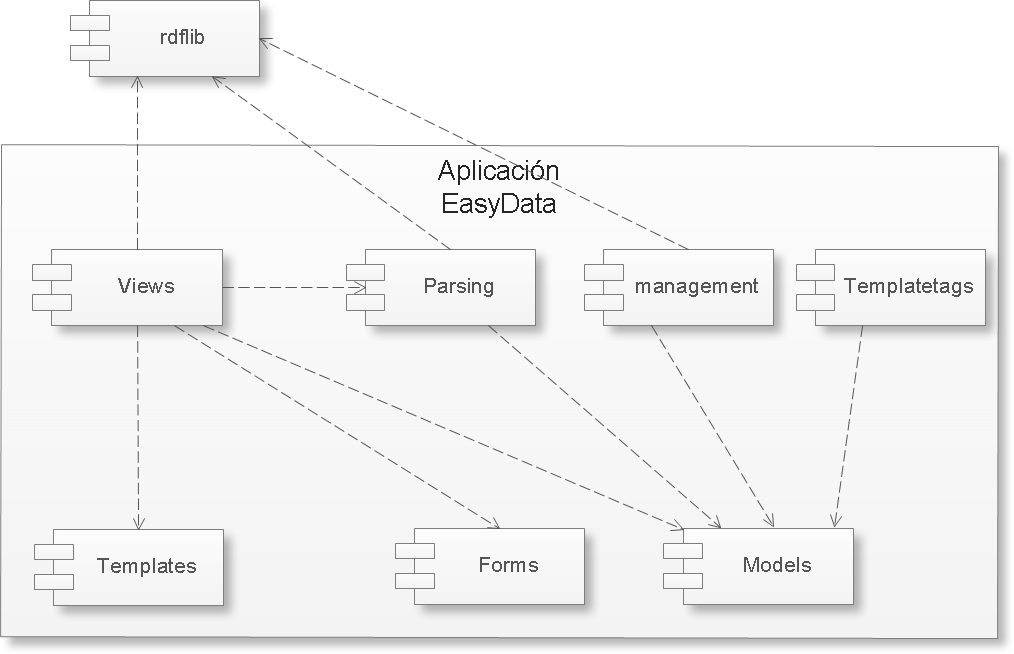
\includegraphics[width=1.05\textwidth]{disenio/modelo_componentes.png}
    \end{center}
    \caption{Estructura de los componentes de la aplicación}
    \label{fig:componentes}
\end{figure}

Donde cada uno de los componentes que se aprecian en la figura
\ref{fig:componentes} son los encargados de realizar las siguientes
funcionalidades:
\begin{itemize}
    \item \textbf{Views:} Almacena todas las vistas de django
        (controladores en el patrón MVC) de los que estará compuesto la
        aplicación, y está dividido en submódulos según la funcionalidad que
        realiza cada uno de la siguiente forma:
    \begin{itemize}
        \item \textbf{map:} almacena aquellas vistas encargadas de realizar el
            mapeo entre los modelos y entidades y entre los fields y
            propiedades.
        \item \textbf{modelo:} almacena las vistas encargadas de configurar la
            visibilidad de los modelos y sus fields.
        \item \textbf{namespaces:} contiene las vistas encargadas de la gestión
            de los namespaces, tanto la alta, edición como eliminado de un
            namespace.
        \item \textbf{publish:} contiene aquellas vistas encargadas de realizar
            la publicación de los datos según el mapeo realizado de los mismos.
        \item \textbf{sesiones:} contiene las vistas encargas de realizar tanto
            el login como el logout de la aplicación.
    \end{itemize}
    \item \textbf{management:} contiene aquellos comandos que se añadirán al
        manage.py de Django. En este caso, se trata de loadmodels y de
        easydata\_d2rq, que se encargará de realizar la captación de los modelos
        y fields del proyecto Django y de generar el fichero de configuración
        para d2rq, respectivamente.
    \item \textbf{Models:} contiene cada uno de los modelos definidos para la
        aplicación EasyData. Cada uno de los módulos de los que está compuesto,
        contiene cada uno de los modelos con el mismo nombre que indica el
        módulo.
    \item \textbf{Template tags:} contiene aquellas funciones que se usarán en
        las plantillas Django para la publicación de información. Está separado
        en dos módulos easydata\_microdata y easydata\_rdfa, para la publicación
        en los formatos en microdata y rdfa respectivamente. Los template tags,
        hacen uso de los modelos para obtener los datos que van a publicar.
    \item \textbf{Parsing:} Contiene aquellas clases y funciones encargadas de
        realizar el parseo de los ficheros RDF (o cualquier otro formato que se
        desee añadir en un futuro) para la carga de nuevos namespaces.
    \item \textbf{Templates:} contiene todas las plantillas donde los
        controladores (vistas de Django), renderizan los datos generados. Estos
        estarán compuestos principalmente por plantillas html.
    \item \textbf{forms:} este componente o módulo de la aplicación contiene
        todos los formularios django que se usarán en las vistas.
    \item \textbf{rdflib:} es un módulo externo que se usará en el proyecto, el
        cuál ofrece funciones para el tratamiento de ficheros RDF.
\end{itemize}

Para plasmar la funcionalidad que tienen cada uno de los componentes que
integran la aplicación, vamos a utilizar diagramas de interacción, donde se
podrá observar como se combinan cada uno de estos para proporcionar una
determinada funcionalidad. Estos elementos no se corresponderán únicamente con
los datos especificados en el diagrama anterior, sino que además podrán verse el
resto de componentes software que intervienen en la prestación de una
determinada funcionalidad. Estas funcionalidades, se corresponderán con aquellas
que hemos descrito en apartados anteriores.

\subsection{Diagramas de interacción}

A continuación mostramos los diagramas de interacción correspondientes a cada
una de las funcionalidades que hemos descrito, las cuales debe de cumplir el
proyecto.
\newpage
\subsubsection{Carga de modelos del proyecto}

\begin{figure}[H]
    \begin{center}
        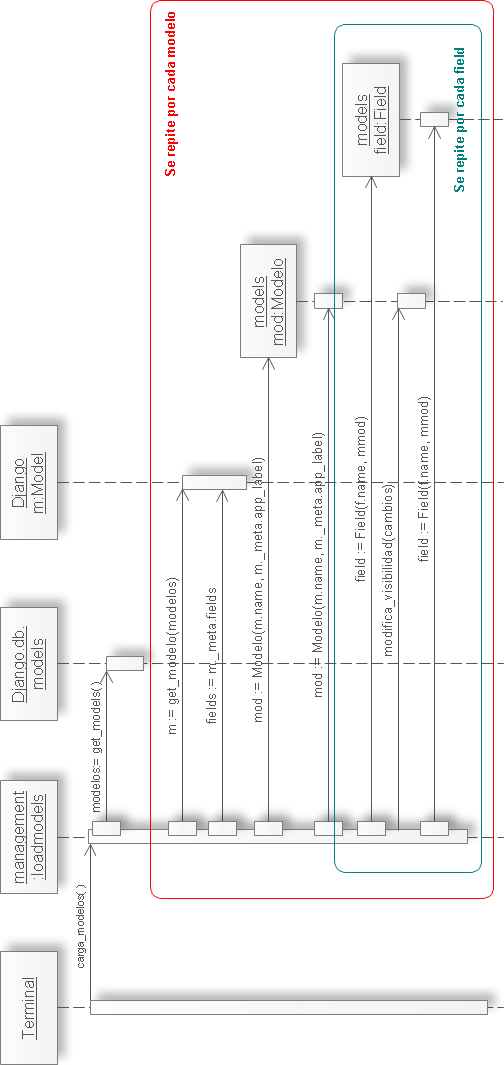
\includegraphics[width=0.62\textwidth]{disenio/interaccion/carga_modelos.png}
    \end{center}
    \caption{Diagrama de interacción: carga de modelos del proyecto}
    \label{fig:carga_modelos}
\end{figure}

\newpage

\subsubsection{Carga de namespaces}

\begin{figure}[H]
    \begin{center}
        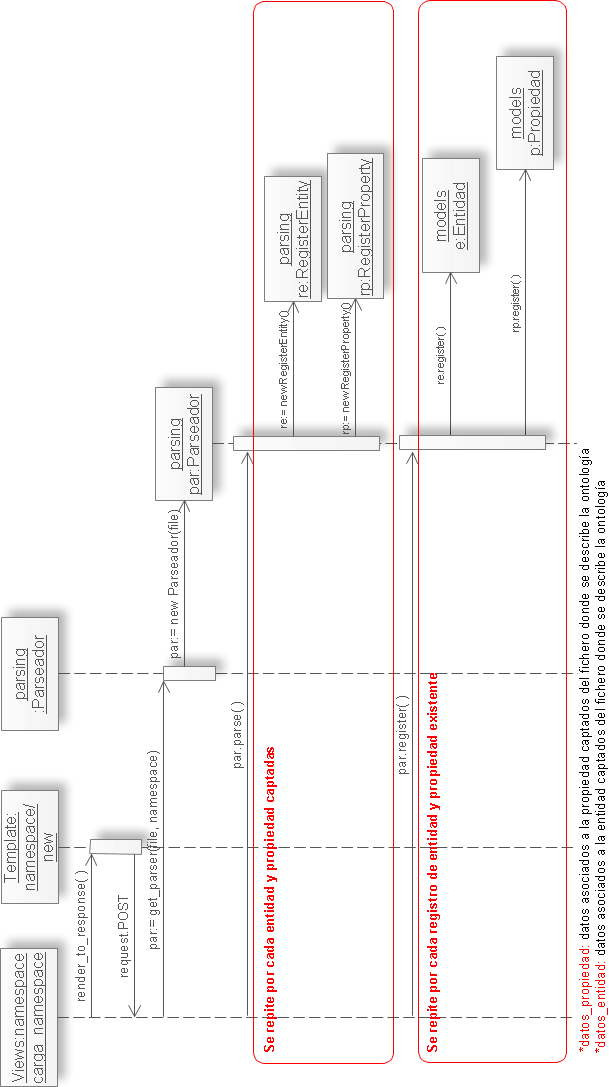
\includegraphics[width=0.65\textwidth]{disenio/interaccion/carga_namespace.png}
    \end{center}
    \caption{Diagrama de interacción: carga de namespaces}
    \label{fig:carga_namespace}
\end{figure}

\newpage

\subsubsection{Configuración de la visibilidad}

\begin{figure}[H]
    \begin{center}
        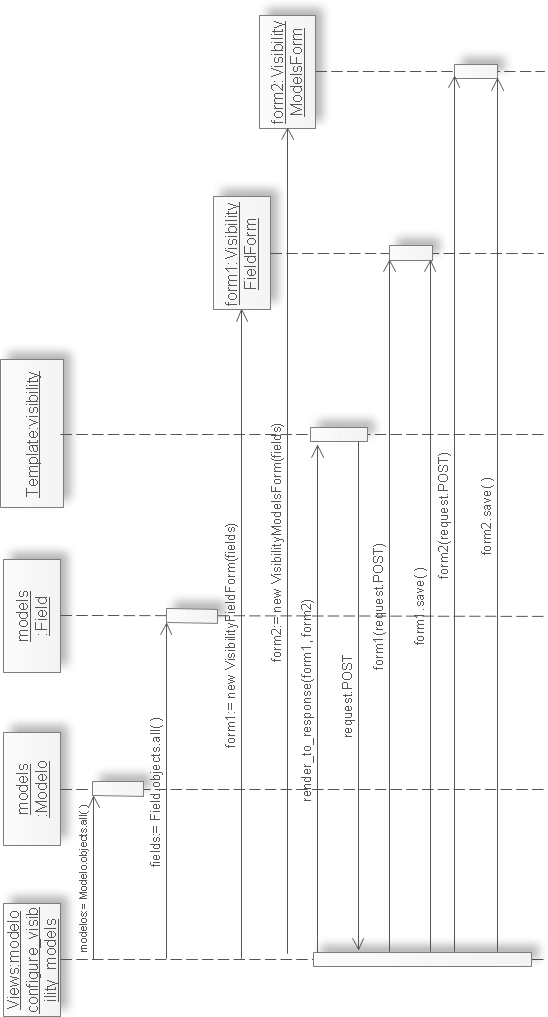
\includegraphics[width=0.7\textwidth]{disenio/interaccion/configurar_visibilidad.png}
    \end{center}
    \caption{Diagrama de interacción: configuración de la visibilidad}
    \label{fig:configura_visibilidad}
\end{figure}

\newpage

\subsubsection{Mapeo de los modelos del proyecto}

\begin{figure}[H]
    \begin{center}
        \includegraphics[width=0.7\textwidth]{disenio/interaccion/mapeo_modelos.png}
    \end{center}
    \caption{Diagrama de interacción: mapeo de los modelos del proyecto}
    \label{fig:mapeo_modelos}
\end{figure}

\newpage

\subsubsection{Mapeo de los atributos de los modelos}

\begin{figure}[H]
    \begin{center}
        \includegraphics[width=0.7\textwidth]{disenio/interaccion/mapeo_atributos.png}
    \end{center}
    \caption{Diagrama de interacción: mapeo de los atributos de los modelos}
    \label{fig:mapeo_atributos}
\end{figure}

\newpage

\subsubsection{Publicación de datos}

\begin{figure}[H]
    \begin{center}
        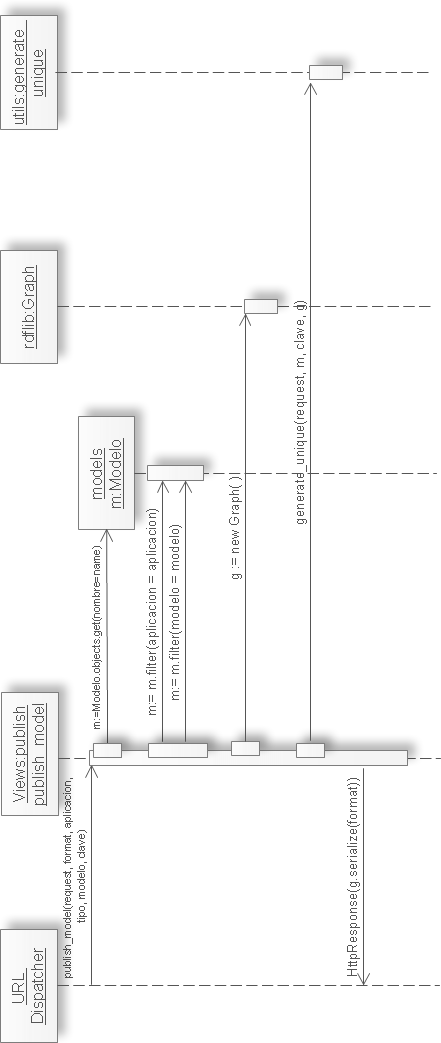
\includegraphics[width=0.58\textwidth]{disenio/interaccion/publicar_datos_element.png}
    \end{center}
    \caption{Diagrama de interacción: publicación de datos para un elemento determinado}
    \label{fig:publicar_datos_element}
\end{figure}

\newpage

\begin{figure}[H]
    \begin{center}
        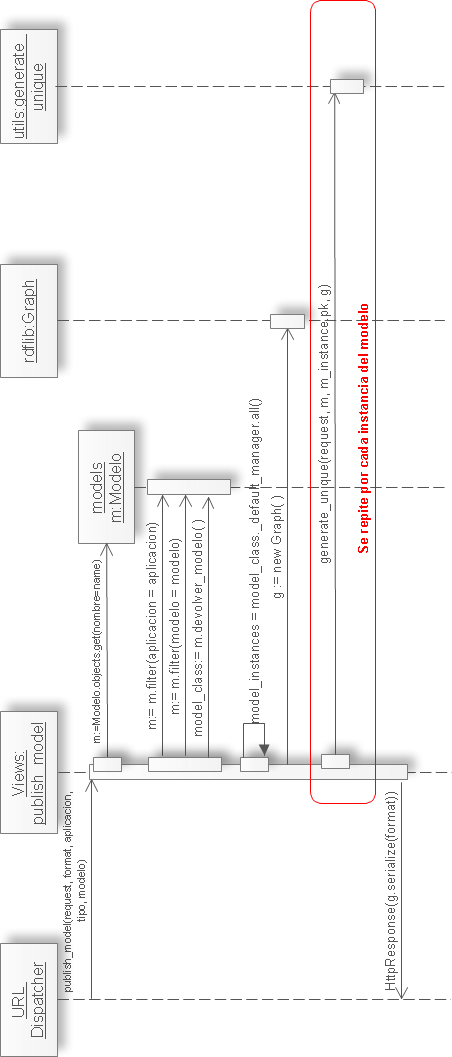
\includegraphics[width=0.6\textwidth]{disenio/interaccion/publicar_datos_model.png}
    \end{center}
    \caption{Diagrama de interacción: publicación de datos para todos los elementos de un modelo}
    \label{fig:publicar_datos_model}
\end{figure}

\newpage

\begin{figure}[H]
    \begin{center}
        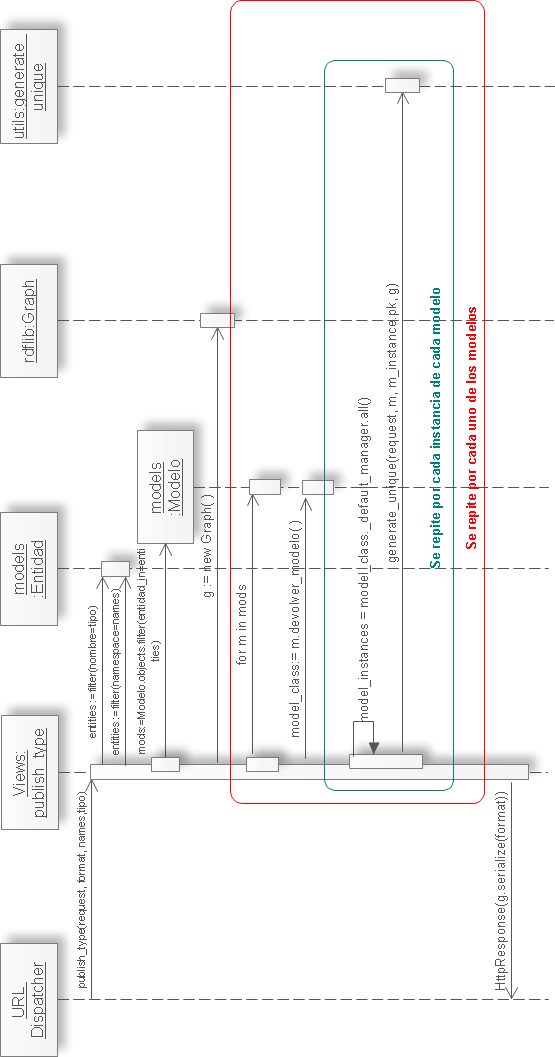
\includegraphics[width=0.7\textwidth]{disenio/interaccion/publicar_datos_type.png}
    \end{center}
    \caption{Diagrama de interacción: publicación de datos para todos los elementos de un tipo}
    \label{fig:publicar_datos_type}
\end{figure}

\newpage

\begin{figure}[H]
    \vspace{4cm}
    \begin{center}
        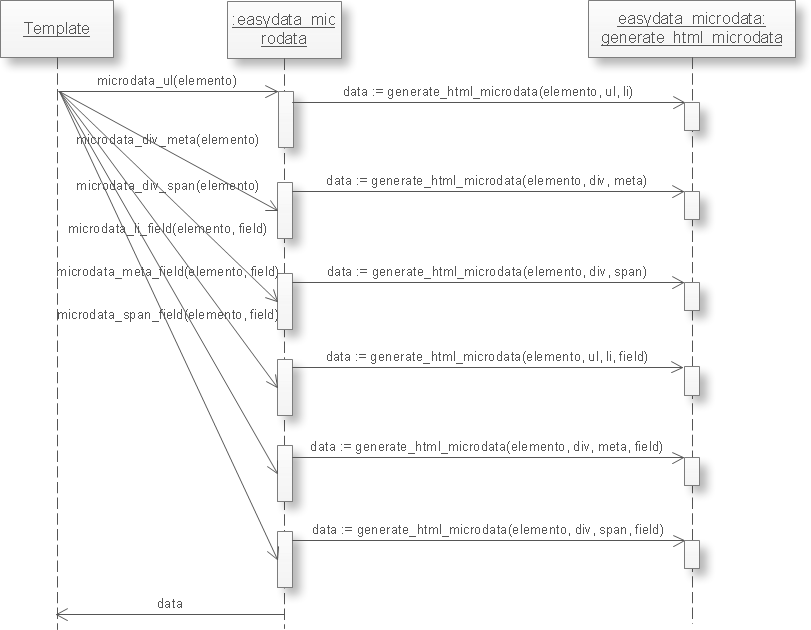
\includegraphics[width=1\textwidth]{disenio/interaccion/publicar_datos_microdata.png}
    \end{center}
    \caption{Diagrama de interacción: publicación de datos mediante microdata}
    \label{fig:publicar_datos_microdata}
\end{figure}

\newpage

\begin{figure}[H]
    \vspace{2cm}
    \begin{center}
        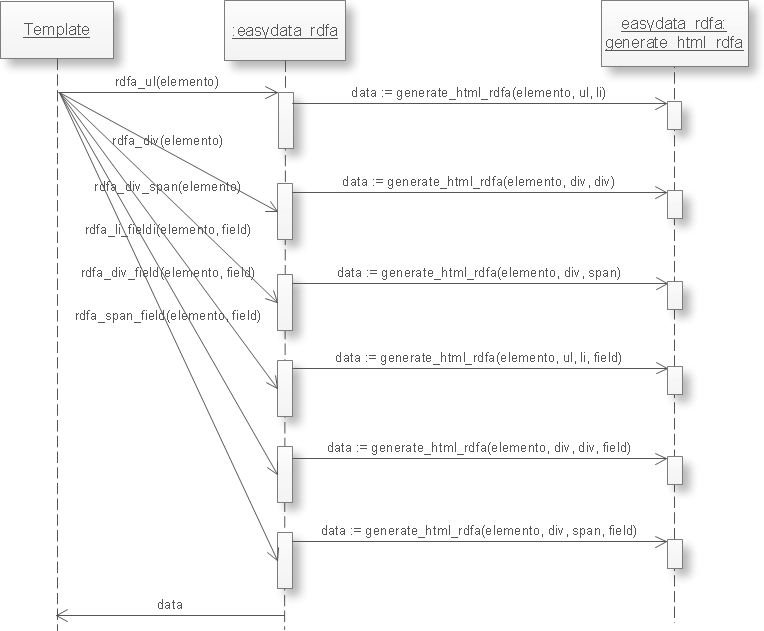
\includegraphics[width=1\textwidth]{disenio/interaccion/publicar_datos_rdfa.png}
    \end{center}
    \caption{Diagrama de interacción: publicación de datos mediante rdfa}
    \label{fig:publicar_datos_rdfa}
\end{figure}

\subsubsection{Generación fichero D2Rq}

\begin{figure}[H]
    \begin{center}
        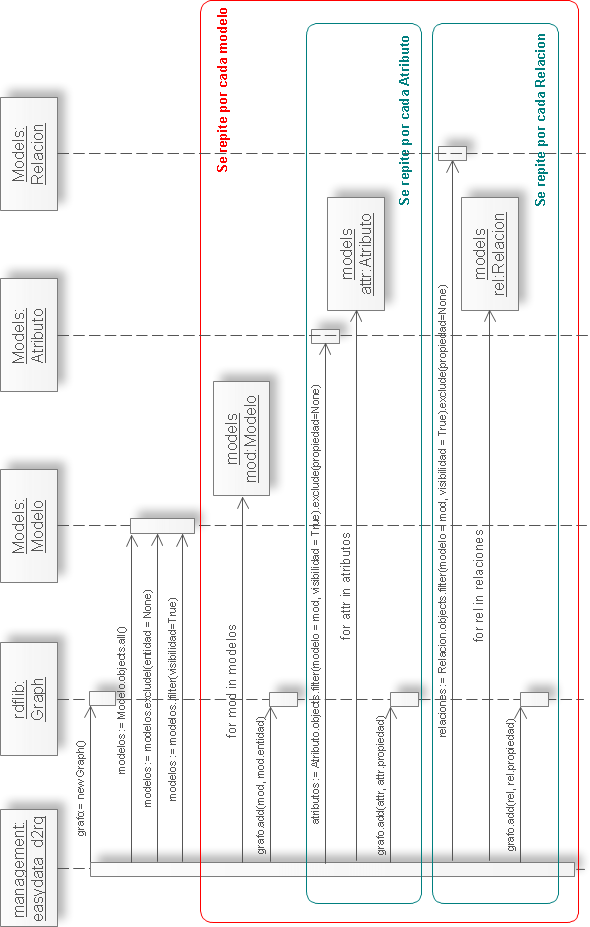
\includegraphics[width=0.8\textwidth]{disenio/interaccion/d2rq.png}
    \end{center}
    \caption{Diagrama de interacción: generación de fichero d2rq}
    \label{fig:d2rq}
\end{figure}

%Para cada uno de los módulos funcionales del sistema debemos realizar un diagrama de secuencia, para definir la interacción existente entre las clases de objetos que permitan responder a eventos externos. A partir de este diagrama, se genera el diagrama de clases de diseño, incluyendo los elementos del modelo conceptual, enriquecidos con las nuevas clases, relaciones, atributos y operaciones resultantes. Asimismo, se detallará el comportamiento de las operaciones más relevantes.
